\section*{Learning Objectives}
\begin{itemize}
\item Learn one way to assign a notion of length to a vector
\item The concept of finding approximate solutions to $Ax=b$ when an exact solution does not exist and why this is extremely useful in engineering.
\end{itemize}

\section*{Outcomes}
\begin{itemize}
\item Euclidean norm and its properties
\item If $Ax=b$ does not have a solution, then for any $x \in \real^n,$ the vector $Ax-b$ is never zero. We will call $e:=Ax-b$ the error vector and search for the value of $x$ that minimizes the norm of the error vector.
\item An application of this idea is Linear Regression, one of the ``super powers'' of Linear Algebra: fitting functions to data.
\end{itemize}


\vspace*{2cm}

\newpage

\section{Norm or ``Length'' of a Vector}
%\textbf{Section 4.4 in Kuttler}

% \includegraphics[scale=0.90,trim={1cm 21cm 0cm 3.7cm},clip, page=170]{PDFofKuttler/Kuttler2017A.pdf}

\begin{tcolorbox}[title=\textbf{Definition: The norm of a vector in $\boldsymbol{\real^n}$}]
Let $v=\begin{bmatrix} v_1 \\ v_2 \\ \vdots \\ v_n  \end{bmatrix} $ be a vector in $\real^n$. The \textbf{Euclidean norm} of $v$, denoted $||v||$, is defined as
\begin{equation}
    \label{eq"DefEuclideanNorm}
    ||v||:=\sqrt{(v_1)^2 + (v_2)^2 + \cdots + (v_n)^2}
\end{equation}
\mbox{ }
\end{tcolorbox}

\vspace*{0.2cm}

\textbf{Example:} The length of the vector $v=  \left[ \begin{array}{r} \sqrt{2} \\ -1 \\ 5   \end{array} \right] $ is
$$ ||v||:=\sqrt{ (\sqrt{2})^2 + (-1)^2 + (5)^2 } = \sqrt{ 2 +1 + 25 } =\sqrt{28} = \sqrt{ 4 \cdot 7} = 2 \sqrt{7} \approx 5.29. $$


\vspace*{0.5cm}
\begin{tcolorbox}[sharp corners, colback=green!30, colframe=green!80!blue, title=\textbf{\large Properties of the Norm of a vector}]
Let's get used to term \textbf{norm of a vector}, which is the correct mathematical term for the length of a vector. There are actually many different ways of defining a notion of ``length'' to a vector. The particular norm defined in Definition 4.14 is the ``Euclidean norm.'' All norms satisfy the following properties 
\begin{itemize}
    \item For all vectors $v \in \real^n$, $||v|| \ge 0$ and moreover, $||v||=0 \iff v=0$. 
    \item For any real number $\alpha \in \real$ and vector $v \in \real^n$, $$||\alpha v|| = |\alpha| \cdot ||v||.$$
    \item For any pair of vectors $v$ and $w$ in $\real^n$,
$$ ||v + w|| \le ||v|| + ||w||. $$
\end{itemize}

\vspace*{0.5cm}
The first property says that $v$ has norm zero if, and only if, $v$ is the zero vector. It seems pretty obvious for our notion of norm and it is!\\


For the second property, we note that we have to take the absolute value of the constant when we ``factor it out'' of the norm. This is because $\sqrt{a^2} = |a|$ and NOT $a$ when $a < 0$. Of course, when $a \ge 0$, $\sqrt{a^2} = a$.\\

The third property is often called the \textbf{triangle inequality}. It says that the norm of a sum of vectors is upper bounded by the sum of the norms of the individual vectors. Another way to say this is, ``the length of $v + w$ can never be strictly larger than the length of $v$ plus the length of $w$.'' What happens if you have $||v-w||$? Well,
\begin{equation}    
\label{eq:TriagIneqJWG}
\begin{aligned}
    ||v-w|| & = ||v + (-w)|| \\
    & \le ||v|| + ||-w|| \\
    & = ||v|| + |-1|\cdot ||w|| \\
    & = ||v|| + ||w||.
\end{aligned}
\end{equation}
Hence, a minus sign changes nothing!

\end{tcolorbox}

\vspace*{0.2cm}

\textbf{Remark:} Equation \ref{eq:TriagIneqJWG} is correct with the ``equals sign'' in the last two equations because $||v|| + ||-w|| = ||v|| + |-1|\cdot ||w||$ and $||v|| + |-1|\cdot ||w|| = ||v|| + ||w||$. Some authors would carry the ``less than or equal to symbol'' all the way through. With our notation, you know where the upper bounding took place!

\vspace*{0.5cm}
\textbf{Example} We'll take three vectors in $\real^4$ and check the ``triangle inequality.'' 
$$ u=  \left[ \begin{array}{r} 2 \\ -1 \\ 5 \\ 2  \end{array} \right],  v=  \left[ \begin{array}{r} 1 \\ 2 \\ 0 \\ 3   \end{array} \right],  w=  \left[ \begin{array}{r} 0 \\ 1 \\ 0 \\4   \end{array} \right] $$

We first compute the norms of the three vectors
$$||u|| = \sqrt{34}\approx 5.83,  ||v|| = \sqrt{14} \approx 3.74, ||w||=\sqrt{17
} \approx 4.12$$
and we then form a few sums against which to test the triangle inequality
$$ u + v = \left[ \begin{array}{r} 3 \\ 1 \\ 5 \\ 5   \end{array} \right], u + v + w = \left[ \begin{array}{r} 3 \\ 2 \\ 5 \\ 9   \end{array} \right], v+w =   \left[ \begin{array}{r} 1 \\ 3 \\ 0\\ 7   \end{array} \right].$$

Then we can check that
\begin{align*}
    ||u+v|| &= \sqrt{60} \approx 7.75 \le  5.8 + 3.7 \le ||u|| + ||v|| \\
    ||u+v+w||&= \sqrt{119} \approx 10.91 \le 7.7 + 4.1 \le ||u+v|| + ||w|| \\
    ||u+v+w||&= \sqrt{119} \approx 10.91 \le 5.8 + 3.7 + 4.1 \le||u|| + ||v|| + ||w||
\end{align*}  


% \section{Removed for now:unit vector, distance between two vectors and the dot product}
% This material is still in Version 01 of this Chapter. In the Junk Folder:\\
% \textbf{VectorSpaceMaterialv01.tex}

\section{Least Squared Error Solutions to Linear Equations}
\label{sec:LeastSqauresGeneral}

In this section, we tackle the problem of providing a notion of ``best approximate solution'' to a system of linear equations that does not have an exact solution. If the system of equations does have an exact solution, our approximate solution will be identical to it. Hence, our development can be viewed as an alternative means of defining solutions to linear equations. 

Consider a system of linear equations $Ax=b$ and define the vector
\begin{equation}
\label{eq:errorDef}
    e(x):=Ax-b
\end{equation}
as the \textbf{error in the solution} for a given value of $x$. Normally, we'll simply write $e:=Ax-b$, but in \eqref{eq:errorDef}, we are emphasizing that the error really is a function of $x$. Hence, as we vary $x$, the ``length'' of $e(x)$ can become bigger or smaller. \\

If the system of equations $Ax=b$ has a solution, then it is possible to make the error zero. In the previous section, we introduced the Euclidean norm as a means of measuring the ''length'' of a vector. It is traditional when posing the best approximation problem to use the square of the norm instead of the norm itself, which means we are simply removing the square root operation in the formula for a norm.

\begin{tcolorbox}
\textbf{Least Squared Error Solution:} Consider a linear system of equations expressed in matrix form $Ax-b$, where $A$ is $n \times m$, $x$ is $m \times 1$ and $b$ is $n \times 1$. For a given value of $x\in \real^m$, define the error as in \eqref{eq:errorDef}, an $n \times 1$ vector. The norm squared of the error vector $e(x)$ is then
\begin{equation}
    \label{eq:LeastSquaredError}
    ||e(x)||^2 := \sum_{i=1}^{n} (e_i(x))^2= e(x)^\top e(x) = (Ax-b)^\top (Ax-b)=|| Ax-b||^2.
\end{equation}
We note that $||e(x)||^2 \ge 0$ for any $x \in \real^m$ and hence zero is a lower bound on the norm squared of the error vector. A value $x^\ast \in \real^m$ is a \textbf{Least Squared Error Solution} to $Ax=b$ if it satisfies
% \min_{x \in \real^m} ||e(x) ||^2 = 
\begin{equation}
    \label{eq:DefLeastSqaredErrorSolution}
    ||e(x^\ast)||^2 = \min_{x \in \real^m} ||Ax-b ||^2
\end{equation}
If such an $x^\ast \in \real^m$ exists and is unique, we will write it as 
\begin{equation}
    \label{eq:DefArgMinLeastSqaredErrorSolution}
    x^\ast := \argmin_{x \in \real^m} ||Ax-b ||^2.
\end{equation}
With this notation, the value of $x$ that minimizes the error in the solution is what is returned by the function $\argmin$, while the minimum value of the error is what is returned by the function $\min$,
\begin{itemize}
    \item $x^\ast = \argmin_{x \in \real^m} ||Ax-b ||^2$ is the value of $x$ that achieves the minimum value of the squared norm of the error, $||Ax-b||^2$, while
    \item $||e(x^\ast)||^2 = ||Ax^\ast - b||^2 = \min_{x \in \real^m} ||Ax-b ||^2$ is the minimum value of the ``squared approximation error''.
\end{itemize}

\end{tcolorbox}


If $Ax=b$ has a solution, then 
$$\min_{x \in \real^m} ||Ax-b ||^2 = 0, $$
because the norm squared error cannot be negative; indeed, zero is the smallest possible value. Hence, while we are most interested in cases where $Ax=b$ does not have a solution, if it does have a unique solution $\bar{x}$ such that $A\bar{x}=b$, then
$$\bar{x} = x^\ast := \argmin_{x \in \real^m} ||Ax-b ||^2 .$$
We recall that uniqueness of solutions to $Ax=b$ is tied to the columns of $A$ being linearly independent. Let's also observe that if $Ax=b$, then 
\begin{itemize}
    \item multiplying both sides of $Ax=b$ by $A^\top$ gives
$$A^\top \cdot  A x = A^\top \cdot b. $$
\item The indicated matrix multiplications are well defined because $A^\top$ is $m \times n$, $A$ is $n \times m$, and $b$ is $n \times 1$. 
\item $A^\top \cdot  A$ is therefore square and $m \times m$.
\item $A^\top \cdot  A$ is symmetric because 
$$\left( A^\top \cdot  A\right)^\top = A^\top \cdot \left(A^\top \right)^\top =A^\top \cdot  A $$
because $\left(A^\top \right)^\top = A.$
\end{itemize}



\begin{tcolorbox}[sharp corners, colback=green!30, colframe=green!80!blue, title=\textbf{\large Least Squared Error Solutions to Linear Equations}]
Here are the main results on solutions to $Ax=b$ that minimize the squared error $||Ax-b||^2$.
\begin{enumerate}
\renewcommand{\labelenumi}{(\alph{enumi})}
\setlength{\itemsep}{.2cm}

\item $A^\top A$ is invertible if, and only if, the columns of $A$ are linearly independent.

\item If $A^\top A$ is invertible, then there is a unique vector $x^\ast \in \real^m$ achieving $\min_{x \in \real^m } ||Ax-b ||^2$ and it satisfies the equation
\begin{equation}
    \label{eq:LeastSquaresSolution}
    \left(A^\top A \right) x^\ast = A^\top b.
\end{equation}
\item Therefore, if $A^\top A$ is invertible, 
\begin{equation}
    \label{eq:ThmLeastSqaredErrorSolution}
  x^\ast = (A^\top A)^{-1} A^\top b  \iff  x^\ast = \argmin_{x \in \real^m} ||Ax-b ||^2 \iff \left(A^\top A \right) x^\ast = A^\top b.
\end{equation}
\end{enumerate}
As you might guess by now, your instructors prefer that for large systems of equations, you solve \eqref{eq:LeastSquaresSolution} to obtain the least squares solution and avoid doing the inverse. For small systems, we'll cut you some slack.\\

\textbf{Useful Remark:} Suppose that $A$ is a ``tall matrix'' (more rows than columns) and suppose that $Ax=b$ has a solution (hence, $b$ is a linear combination of the columns of $A$). Then, if the columns of $A$ are linearly independent, you can compute the solution using \eqref{eq:LeastSquaresSolution} and the squared error will be zero, meaning $x^\ast$ really is a solution to the equation because $$\text{the squared error is zero} \iff ||A x^\ast - b||^2 = 0 \iff ||A x^\ast - b|| = 0 \iff A x^\ast - b=0 \iff A x^\ast = b.$$ 
Try it on your own in Julia!
\end{tcolorbox}

\vspace*{0.2cm}

\begin{example}
\label{ex:LeastSqauredLinearEquations}
Let's consider a system of linear equations, with more equations than unknowns. The extra equations provide more conditions that a solution must satisfy, making non-existence of a solution a common occurrence! We take
\begin{equation}
\label{eq:LeastSquareSolExample}
\underbrace{\left[\begin{array}{rrr}
 1.0 & 1.0 \\
 2.0 & 1.0 \\
 4.0 & 1.0 \\
 5.0 & 1.0 \\
 7.0  & 1.0
 \end{array}\right]}_{A} \underbrace{\left[\begin{array}{c}
x_1 \\ x_2  \end{array}\right]}_{x} =  \underbrace{\left[\begin{array}{r}
4 \\  8 \\ 10 \\ 12 \\ 18 \end{array}\right]}_{b},
\end{equation}
and note that the columns of $A$ are linearly independent. If a regular solution exists, find it. If not, then a least squared solution will be fine.
\end{example}

\textbf{Solution:} 
We'll compute a least squared error solution to the equations, and then we'll evaluate the error; if the error is zero, we'll also have an exact solution to \eqref{eq:LeastSquareSolExample}. We compute 
$$A^\top \cdot A = \left[\begin{array}{rr} 
95.0 & 19.0 \\
19.0  &  5.0 \end{array}\right],~
A^\top \cdot b = \left[\begin{array}{r} 
246.0\\
  52.0 
  \end{array}\right] \implies x^\ast= 
  \left[\begin{array}{r} 
  2.12 \\
 2.33 
 \end{array}\right]$$
For the record, $\det(A^\top \cdot A)=114.$ We also compute
$$e^\ast:=Ax^\ast-b = \left[\begin{array}{r}
0.456\\
 -1.421\\
  0.825 \\
  0.947\\
 -0.807 
 \end{array}\right], ~||e||=2.111,~\text{and}~ ||e||^2 = 4.456 $$
 Because the ``smallest'' error vector $e^\ast=Ax^\ast-b$ is non-zero, we now know that \eqref{eq:LeastSquareSolExample} does not have an exact solution. 
 Next, we take a new vector $b=\left[
\begin{array}{c}
0.30 \\
1.00 \\
2.40 \\
3.10\\
4.50 \\
\end{array}
\right]$ and check if there is an exact solution or not. We proceed in the same manner and solve $A^\top \cdot A x^\ast =A^\top b$ and compute 
$$ x^\ast = \left[
\begin{array}{r}
0.7000 \\
-0.4000 \\
\end{array}
\right] \text{ and } e:= A x^\ast - b = \left[
\begin{array}{c}
0.0000 \\
0.0000 \\
0.0000 \\
0.0000 \\
0.0000 \\
\end{array}
\right],$$
and hence for this new vector $b$, the rectangular system $Ax = b$ has an exact solution. Moreover, we found it by applying our theory for least squared error solutions to overdetermined equations, which is pretty nifty!
  \Qed\\
  
The set of linear equations \eqref{eq:LeastSquareSolExample} and its solution look rather ho hum. They are actually anything but boring. Figure~\ref{fig:MotivatingLeastSqaures} shows that the equations and their solution correspond to fitting a line through data, while minimizing the ``fitting error''! In the next section, we will develop this idea thoroughly and give you a hint of some of the things you can do with least squared error solutions to linear equations. 
\begin{figure}[!hbt]
        \centerline{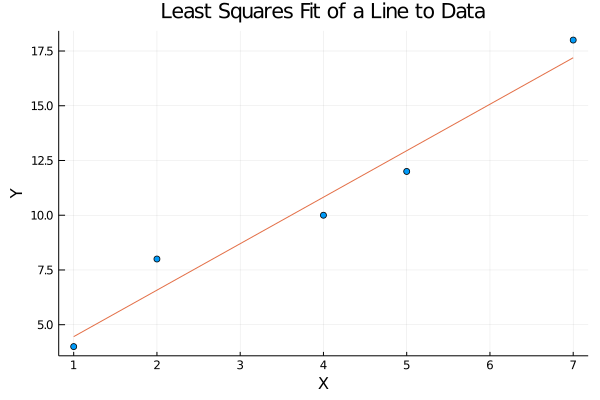
\includegraphics[scale=0.5]{Chap08NormLinearRegression/dataSet1WithLine.png}}
        \caption{The physical basis for the numbers in \eqref{eq:LeastSquareSolExample}, which is really about fitting a line to data with minimum squared error! The dots are the $(x,y)$ values of the raw (measured) data, while the line is a model that summarizes the data in the form $y=m x + b$. One important aspect of the model is that you can now predict values of $y$ for values of $x$ that you did not directly measure. This is called interpolation when $x$ is within the limits of the measured data (here, $1 \le x \le 7$) and extrapolation otherwise. }
        \label{fig:MotivatingLeastSqaures}
\end{figure}

\section{Linear Regression or Fitting Functions to Data}
\label{sec:LinearRegression}



The goal of this section is explain how to fit functions to data. The following is a prototypical problem: given the data shown in Table \ref{tab:LinearData}, which is also plotted in Fig.~\ref{fig:PlotLinearData}, find a function that explains the data.\\

It is clear that the data do NOT lie exactly on a straight line. How can we {\bf approximately} fit a straight line to the data? In particular, how can we find a function that minimizes a meaningful sense of fitting error to the data?

\begin{table}[!hbt]
\caption[]{Data for our first fitting problem.}
\label{tab:LinearData}
%\spacing 1
\begin{center}
\begin{tabular}{||c|c|c||}
\hline
$ i$ & $x_i$ & $y_i$\\
\hline
1 &1  &   4 \\
 2& 2    &  8 \\
3& 4   & 10 \\
4& 5  &  12 \\
5 & 7   & 18 \\
\hline
\end{tabular}
\end{center}
%\spacing 2
\end{table}

\begin{figure}[!hbt]
        \centerline{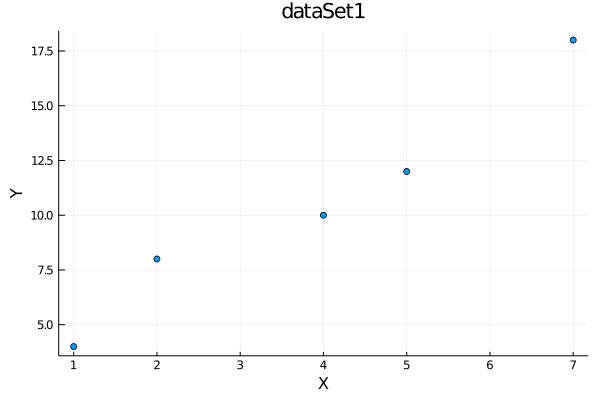
\includegraphics[scale=0.5]{Chap08NormLinearRegression/dataSet1.png}}
        \caption{Plot of data in Table~\ref{tab:LinearData}}
        \label{fig:PlotLinearData}
\end{figure}
Let's suppose that we wish to fit a linear model  $\hat{y}=mx+b$ to the data, which has been plotted in Fig.~\ref{fig:PlotLinearData}. We set up the linear equations
$$y_i = m x_i +b = \begin{bmatrix} x_i & 1 \end{bmatrix} \begin{bmatrix} m \\ b \end{bmatrix},  ~~1 \le i \le N,$$ 
where $N$ is the number of data points (five in the case of Table~\ref{tab:LinearData}), and write it out in matrix form
\begin{equation}
    \label{eq:FirstRegressionModel02}
\underbrace{\begin{bmatrix} y_1 \\ y_2 \\ \vdots \\y_N \end{bmatrix}}_{Y} = \underbrace{\left[\begin{array}{cc}
    x_1 & 1 \\
    x_2  & 1 \\
    \vdots & 1 \\
    x_N & 1
\end{array}  \right]}_{\Phi} \cdot  \underbrace{\begin{bmatrix} m \\ b \end{bmatrix}}_{\alpha},
\end{equation}
where $Y$ is the vector of $y$-data, $\Phi$ is called the \textbf{regressor matrix} and $\alpha$ is the vector of \textbf{unknown coefficients} that parameterize the  model.

From the data in Table~\ref{tab:LinearData}, the matrices are
$$ Y= \left[\begin{array}{r}
4 \\  8 \\ 10 \\ 12 \\ 18 \end{array}\right], ~ \Phi=  \left[\begin{array}{rr}
 1.0 & 1.0 \\
 2.0 & 1.0 \\
 4.0 & 1.0 \\
 5.0 & 1.0 \\
 7.0  & 1.0
 \end{array}\right], ~\text{and} ~ \alpha= \left[\begin{array}{r}
m\\
b
 \end{array}\right].$$
 $Y$ is the vector of ``measured'' $y$-values. $\alpha$ is the vector of unknown coefficients that we seek to estimate. $\Phi$,  the regressor matrix, is defined so that the $i$-th row of $Y=\Phi \alpha$ corresponds to $y_i=m x_i + b.$ \\
 
 The fitting error will be $e_i = y_i-(m x_i + b)$, which when written as a vector gives 
$$ \underbrace{\left[\begin{array}{r}
e_1\\ e_2\\ e_3 \\e_4\\ e_5 \end{array}\right]}_{e} =
\underbrace{ \left[\begin{array}{r}
4 \\  8 \\ 10 \\ 12 \\ 18 \end{array}\right]}_{Y}
-\underbrace{\left[\begin{array}{rr}
 1.0 & 1.0 \\
 2.0 & 1.0 \\
 4.0 & 1.0 \\
 5.0 & 1.0 \\
 7.0  & 1.0
 \end{array}\right]}_{\Phi} \cdot  \underbrace{\left[\begin{array}{r}
m\\
b
 \end{array}\right]}_{\alpha}, $$
 that is, $e:=Y-\Phi \alpha$. We propose to choose the coefficients in $\alpha$ so as to minimize the total squared error
  $$E_{tot} = \sum_{i=1}^{5} (e_i)^2 = e^\top e = ||e||^2= ||Y-\Phi \alpha ||^2.$$
  
\begin{tcolorbox}[sharp corners, colback=green!30, colframe=green!80!blue, title=\textbf{\large Least Squares Fit to Data also called Linear Regression}]

  From Chapter~\ref{sec:LeastSqauresGeneral}, if the columns of $\Phi$ are linearly independent, or equivalently, $\Phi^\top \Phi$ is invertible, then the following are equivalent 
  \begin{equation}
    \label{eq:ThmLeastSqaredErrorSolution2}
  \alpha^\ast = \left( \Phi^\top \Phi \right)^{-1}\Phi^\top Y  \iff  \alpha^\ast = \argmin_{\alpha} ||Y-\Phi \alpha ||^2 \iff \left( \Phi^\top \Phi \right) \alpha^\ast = \Phi^\top Y.
\end{equation}
  
  \end{tcolorbox}
  \vspace*{.2cm}

The associated equations are formulated and solved in the Julia code given below. The plot of the fit is given in Fig.~\ref{fig:MotivatingLeastSqaures}. You can generate your own plots too!
  \vspace*{.2cm}
\UseRawInputEncoding
\begin{lstlisting}[language=Julia]
using Plots
gr()

# Given data
X=[1  2  4  5  7]'
Y=[4  8  10  12  18]'

# Scatter plot
scatter(X,Y)
plot!(xlabel="X", ylabel="Y", title="dataSet1", leg=false)
plot!(fmt = :png)

# Build the regressor matrix
Phi=[X ones(5,1)]
@show Phi

Phi = [1.0 1.0; 2.0 1.0; 4.0 1.0; 5.0 1.0; 7.0 1.0]
5x2 Array{Float64,2}:
 1.0  1.0
 2.0  1.0
 4.0  1.0
 5.0  1.0
 7.0  1.0
 
 # Take a shortcut to finding alpha 
 # because the problem is small
 alphaStar=inv(Phi'*Phi)*Phi'*Y
 2x1 Array{Float64,2}:
 2.1228070175438596
 2.3333333333333375
 
# Extract the physically meaningful parameters 
m=alphaStar[1]
b=alphaStar[2]

# Build the line for plotting
XX=[1, 7]
YY=m*XX.+b
scatter(X,Y)
plot!(xlabel="X", ylabel="Y", title="Least Squares Fit of a Line to Data", leg=false)
plot!(fmt = :png)

# Plot the line over the scatter plot of the data
plot!(XX,YY) 
\end{lstlisting}
  \vspace*{.2cm}

The above shows you how to formulate a least squares fit to data by working through THE CLASSIC EXAMPLE, fitting a line to data by minimizing the total squared error (square of the norm of the error vector). We'll do another example so that you understand that you are not limited to fitting ``linear functions'' to data. 

\begin{table}[!hb]
\caption[]{Data for our second fitting problem.}
\label{tab:QuadraticData}
\begin{center}
\begin{tabular}{||c|l|l||}
\hline
$ i$ & $x_i$ & $y_i$\\
\hline
1 &0  &   1.0 \\
 2& 0.25    &  1.0 \\
3& 0.5   & 1.5 \\
4& 0.75  &  2.0 \\
5 & 1.0   & 3.0 \\
6 & 1.25   & 4.25 \\
7 & 1.5   & 5.5 \\
8 & 1.75   & 7.0 \\
9 & 2.0   & 10.0 \\
\hline
\end{tabular}
\end{center}
\end{table}

\begin{figure}[!hbt]
        \centerline{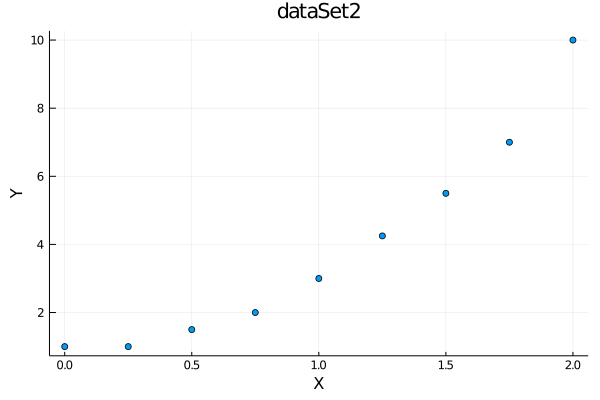
\includegraphics[scale=0.5]{Chap08NormLinearRegression/dataSet2.png}}
        \caption{Scatter plot of the data in Table~\ref{tab:QuadraticData}. The curve looks nonlinear!}
        \label{fig:PlotQuadraticData}
\end{figure}

\begin{example}
\label{ex:FitQuadraticData}
Our method of fitting a line to data is more general than it might seem. Consider the data in Table~\ref{tab:QuadraticData}, which has been plotted in Fig.~\ref{fig:PlotQuadraticData}. It sure doesn't seem like we should fit a line to it. How about a quadratic? 
\end{example}

\textbf{Solution:} Let's choose a model of the form 
$$y=c_0 + c_1 x + c_2 x^2 = \begin{bmatrix} 1 & x & x^2 \end{bmatrix} \begin{bmatrix} c_0 \\ c_1 \\ c_2 \end{bmatrix}.$$ 
Note that even though the model is nonlinear in $x$, it is linear in the unknown coefficients $c_0, ~c_1,~ c_2$. This is what is important!!! Just as before, define $\hat y_i = c_0 + c_1 x_i + c_2 x_i^2$, the $i$-th term of the error vector is then 
$$e_i := y_i - \hat y_i = y_i- (c_0 + c_1 x_i + c_2 x_i^2) $$
and the total squared error is $$E_{tot} = \sum_{i=1}^{N} e_i^2.$$


Writing out the equation $y_i = c_0 + c_1 x_i + c_2 x_i^2$ $,i=1,\cdots,N$ in matrix form yields
$$
\underbrace{\left[ \begin{array}{c} y_1 \\ y_2 \\ \vdots \\ y_N \end{array} \right]}_{Y} =
 \underbrace{\left[ \begin{array}{ccc} 1 & x_1 & (x_1)^2 \\ 1 & x_2 & (x_2)^2 \\ \vdots & \vdots \\ 1 & x_N & (x_N)^2 \end{array} \right]}_{\Phi}
 \underbrace{\left[ \begin{array}{c} c_0 \\ c_1 \\ c_2 \end{array} \right] }_{\alpha},
$$
which gives us the equation $Y = \Phi \alpha$. We plug in our numbers and check that $\det(\Phi^\top \cdot \Phi) = 40.6 \neq 0.$ The resulting fit is given in Fig.~\ref{fig:QuadraticLeastSqaures}. The Julia code is also given.

\begin{figure}[!hbt]
        \centerline{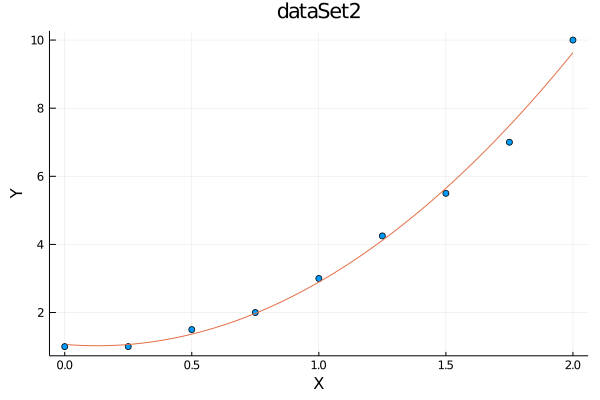
\includegraphics[scale=0.5]{Chap08NormLinearRegression/dataSet2WithCurve.png}}
        \caption{A least squares fit of a quadratic curve, $\hat{y}=c_0 + c_1 x + c_2 x^2$, to data.}
        \label{fig:QuadraticLeastSqaures}
\end{figure}

%\begin{verbatim}
\UseRawInputEncoding
  \begin{lstlisting}[language=Julia]
# Data set
dataSet2=[
1  0.0    1.0 
2  0.25   1.0
3  0.5    1.5
4  0.75   2.0
5  1.0    3.0
6  1.25   4.25
7  1.5    5.5
8  1.75   7.0 
9  2.0   10.0]

# Extract relevant data
X=dataSet2[:,2]
Y=dataSet2[:,3]

# Look at data to see what kind of curve it may be
using Plots
gr()
scatter(X,Y)
plot!(xlabel="X", ylabel="Y", title="dataSet2", leg=false)
plot!(fmt = :png)

# Build the regressor matrix
Phi=[ones(9,1) X  X.^2]
9 x 3 Array{Float64,2}:
 1.0  0.0   0.0
 1.0  0.25  0.0625
 1.0  0.5   0.25
 1.0  0.75  0.5625
 1.0  1.0   1.0
 1.0  1.25  1.5625
 1.0  1.5   2.25
 1.0  1.75  3.0625
 1.0  2.0   4.0

# Solve Regression Problem
alphaStar=inv(Phi'*Phi)*Phi'*Y

# Plot the curve: first way to do it
Yhat=Phi*alphaStar
plot!(X,Yhat)

# Plot the curve with more points in x so that it is smoother
temp=1:200
XX=vec(temp/100.0);
N=length(XX)
PHI=[ones(N,1) XX XX.^2]
#YY=c0.+ c1.*XX + c2.*(XX).^2;
YY=PHI*alphaStar

# Plot used in the notes
scatter(X,Y)
plot!(xlabel="X", ylabel="Y", title="dataSet2", leg=false)
plot!(fmt = :png)
plot!(XX,YY)
\end{lstlisting}
%\end{verbatim}

In HW and in Project 2, we'll explore more refined aspects of regressing functions and surfaces to data. We'll actually divide the data set into two pieces: one to be used for fitting the data and a second portion of the data reserved for checking the quality of the fit. We will be looking to see that the fit to data that was not used in the regression problem is comparable to the fit produced by the regression algorithm. The idea is that the second piece of data better represents how your regressed function (or surface) will work in the real world. \textbf{If you have heard of Machine Learning, these ideas are very close to current practice when ``training'' Supervised Machine Learning Algorithms.} 

\Qed

\begin{tcolorbox}[sharp corners, colback=green!30, colframe=green!80!blue, title=\textbf{\Large Large Scale Least Squares via the LU Factorization}]
 From Chapter~\ref{sec:LeastSqauresGeneral}, if the columns of $\Phi$ are linearly independent, or equivalently, $\Phi^\top \Phi$ is invertible, we know the following are equivalent 
  \begin{equation}
    \label{eq:ThmLeastSqaredErrorSolution2secondTime}
  \alpha^\ast = \left( \Phi^\top \Phi \right)^{-1}\Phi^\top Y  \iff  \alpha^\ast = \argmin_{\alpha} ||Y-\Phi \alpha ||^2 \iff \left( \Phi^\top \Phi \right) \alpha^\ast = \Phi^\top Y.
\end{equation}
The suggested ``pipeline'' for  computing a least squared error solution to $ \left( \Phi^\top \Phi \right) \alpha^\ast = \Phi^\top Y$ is 
\begin{itemize}
    \item factor $P \cdot \left( \Phi^\top \Phi \right)  =: L \cdot U$, that is, do the LU Factorization of $\Phi^\top \cdot \Phi$,
    \item compute $\overline{b}:= P \cdot \Phi^\top Y$, and then 
    \item solve $L y = \overline{b}$ via forward substitution, and
    \item solve $U \alpha^\ast =y$ via backward substitution.
\end{itemize}
\end{tcolorbox}

\begin{tcolorbox}[title={\bf Reminder on Calling LU Correctly in Julia}]
\begin{lstlisting}[language=Julia]
# Find alphaStar by solving Phi' * Y= Phi' * Phi*alphaStar (Ax = b) using LU decomposition
using LinearAlgebra
F = lu(Phi' * Phi)
L = F.L
U = F.U
P = F.P
#
# Phi' * Y = Phi' * Phi * alphaStar
# after LU Factorization of Phi'*Phi, we have
# P *  Phi' * Y  = L * U * alphaStar
# 
y_alpha = forwardsub(L, P*Phi'*Y)
alphaStar = backwardsub(U, y_alpha)
\end{lstlisting}
\vspace*{.2cm}
\textbf{As a reminder, the following is erroneous:}
\vspace*{.2cm}
\begin{lstlisting}[language=Julia]
# Find alphaStar by solving Phi' * Y= Phi' * Phi*alphaStar (Ax = b) using LU decomposition
using LinearAlgebra
L,U,P = lu(Phi' * Phi)
#
y_alpha = forwardsub(L, P*Phi'*Y)
alphaStar = backwardsub(U, y_alpha)
\end{lstlisting}
\textbf{Why?} Because $P$ will NOT contain the permutation matrix. It will contain the list of permutation indices. Give a try!
\end{tcolorbox}


\section{(Optional Read): How to Derive the Main Regression Formula}

The main method is ``completing the square''. You probably learned that in High School when you studied the quadratic formula. We recall first the derivation of the quadratic formula via ``completing the square'' and then give the main steps for a ``vector-matrix version of completing the square.''

\subsection{Completing the Square for the Quadratic Formula:}
We assume that $a\ne 0$ and that all coefficients are real numbers. The main ``trick'' is to recall that $(x+d)^2 = x^2 + 2 dx + d^2$. Hence, if you see something like $x^2 +2 dx$, you can complete the square by adding and subtracting $ d^2$ to obtain $x^2 + 2dx = (x+d)^2 -d^2 $. Below, we do this for $d=\frac{b}{2a}.$
\begin{align*}
    ax^2 + bx + c&=0 \\
    & \Updownarrow  \\
    x^2 + \frac{b}{a}x + \frac{c}{a} & = 0 \\
        & \Updownarrow  \\
    x^2 + 2\frac{b}{2 a}x + \frac{c}{a} & = 0 \\
    & \Updownarrow   \\
       \left( x^2 + 2\frac{b}{2 a}x + \left( \frac{b}{2a}\right)^2\right) - \left( \frac{b}{2a}\right)^2 + \frac{c}{a} & = 0   ~~\text{(the square was completed here!)}
    \end{align*} 
 Really? Yes, because $x^2 + 2\left(\frac{b}{2 a} \right)x + \left( \frac{b}{2a}\right)^2\ = \left(x +   \frac{b}{2a} \right)^2$. Once we have completed the square, the rest is basic manipulation of terms, 
    \begin{align*}
    \left(x +   \frac{b}{2a} \right)^2 & = \left( \frac{b}{2a}\right)^2 - \frac{c}{a} \\
      & \Updownarrow   \\
    \left(x +   \frac{b}{2a} \right)^2 & = \frac{b^2-4ac}{4a^2} ~~\text{(a perfect square)}\\
          & \Updownarrow   \\
    \left(x +   \frac{b}{2a} \right) & = \pm \sqrt{\frac{b^2-4ac}{4a^2}} ~~\text{(note the plus-minus sign)}\\
              & \Updownarrow   \\
    \left(x +   \frac{b}{2a} \right) & = \pm \frac{\sqrt{b^2-4ac}}{2a} ~~\text{(the rest is ``algebra'')}\\
                  & \Updownarrow   \\
x & = -\frac{b}{2a} \pm \frac{\sqrt{b^2-4ac}}{2a} \\
                  & \Updownarrow   \\
x & =  \frac{-b \pm \sqrt{b^2-4ac}}{2a}. 
\end{align*} 
That's a lot of steps. You probably forgot how it went, right? We had to refresh our own thoughts on completing the square.  

\subsection{Completing the Square for Least Squares Solutions to Systems of Linear Equations:} 
Consider the set of equations $Ax=b$ and suppose that the columns of $A$ are linearly independent, or equivalently, that $A^\top A$ is invertible (i.e., $\det(A^\top A) \neq 0$). Then the value of $x$ that minimizes the error satisfies
$$A^\top A x^\ast = A^\top b. $$

\textbf{Sketch:} 
\begin{equation}
    \label{eq:LeastSquaresDerivation}
\begin{aligned}
    ||Ax-b||^2&=(Ax-b)^\top (Ax-b) \\
    &= x^\top A^\top A x -x^\top A^\top b - b^\top A x + b^\top b
\end{aligned}
\end{equation}

This is where completing the square comes in. It is much easier to do if you already know that answer from other techniques! In Linear Algebra, an expression of the form
$$\boxed{\left( A^\top A x - A^\top b \right)^\top \left(A^\top A \right)^{-1}   \left( A^\top A x - A^\top b \right)}$$
 is the equivalent of a perfect square. We expand all the terms 
\begin{align*}
\left( A^\top A x - A^\top b \right)^\top \left(A^\top A \right)^{-1}   \left( A^\top A x - A^\top b \right) &=
    \left(x^\top A^\top A - b^\top A \right) \left(A^\top A \right)^{-1}   \left( A^\top A x - A^\top b \right) \\
    &=  \left(x^\top - b^\top A \left(A^\top A \right)^{-1}\right)  \left( A^\top A x - A^\top b \right) \\
    &= x^\top A^\top A x -x^\top A^\top b -b^\top A x +b^\top A\left(A^\top A \right)^{-1} A^\top b
\end{align*}
and then relate them to the equation we are trying to minimize.\\

Substituting this result into \eqref{eq:LeastSquaresDerivation} gives
\begin{align*}
    ||Ax-b||^2&=(Ax-b)^\top (Ax-b) \\
    &= x^\top A^\top A x -x^\top A^\top b - b^\top A x + b^\top b\\
    &=x^\top A^\top A x -x^\top A^\top b - b^\top A x + b^\top b + b^\top A \left(A^\top A \right)^{-1}  A^\top b- b^\top A \left(A^\top A \right)^{-1}  A^\top b\\
    &=\left( A^\top A x - A^\top b \right)^\top \left(A^\top A \right)^{-1}   \left( A^\top A x - A^\top b \right) +b^\top b - b^\top A \left(A^\top A \right)^{-1}  A^\top b
\end{align*}

% Substituting this result into \eqref{eq:LeastSquaresDerivation} gives
% \begin{align*}
%     ||Ax-b||^2&=(Ax-b)^\top (Ax-b) \\
%     &= x^\top A^\top A x -x^\top A^\top b - b^\top A x + b^\top b\\
%     &=\left(x^\top A^\top A - b^\top A \right) \left(A^\top A \right)^{-1}   \left( A^\top A x - A^\top b \right) +b^\top b - b^\top A \left(A^\top A \right)^{-1}  A^\top b\\
%     &=\left( A^\top A x - A^\top b \right)^\top \left(A^\top A \right)^{-1}   \left( A^\top A x - A^\top b \right) +b^\top b - b^\top A \left(A^\top A \right)^{-1}  A^\top b
% \end{align*}

Here is the \textit{coup de gr\^{a}ce}: We note that $b^\top b - b^\top A \left(A^\top A \right)^{-1}  A^\top b$ does not depend on $x$. Hence, the $x^\ast$ that minimizes \eqref{eq:LeastSquaresDerivation} is that same as the $x^\ast$ that minimizes  
$$ \left( A^\top A x - A^\top b \right)^\top \left(A^\top A \right)^{-1}   \left( A^\top A x - A^\top b \right).$$
Therefore, the solution is
$$\left( A^\top A x^\ast - A^\top b \right)=0 \iff A^\top A x^\ast = A^\top b . $$

\textbf{Remark:} Uniqueness follows because $A^\top A$ is invertible. A more complete derivation would use properties of positive definite matrices that are covered in Appendix~\ref{sec:PosDefMatrices}. 

\section{Looking Ahead}
The next two Chapters will conclude our introduction to Computational Linear Algebra. We want to leave space for covering some nonlinear topics in Chapters \ref{chap:NonlinearEquations} and \ref{chap:Optimization}, topics that are very computational in nature and super useful in engineering practice.\\

Our next chapter will build on our notions of linear combinations and linear independence to introduce a tool, called a dot product, that allows us to study the notion of ``orthogonal vectors'' (also called perpendicular vectors) in $\real^n$ for any $n \ge 2$. You probably recall ``right angles'' from planar geometry? Don't worry, we will not be doing ``similar triangles'' or the ``side-angle-side theorem''. What we will be doing is more on the level of difficulty of the Pythagorean Theorem, $a^2 + b^2 = c^2$. We'll introduce an algorithm that you will want to program up in Julia for constructing orthogonal vectors from a set of linearly independent vectors. And from such vectors, we build matrices that have the amazing property that their inverse is equal to their transpose! We know, it seems too good to be true. And we'll learn how to write any matrix $A$ as the product of one of these magical matrices and an upper triangular matrix.  





